\def\additionalOptionsForClass{nochapname,bigchapter}
\providecommand{\additionalOptionsForClass}{}
\documentclass[
  accentcolor=tud1c,	% Color theme for TUD corporate design
  colorbacktitle,		% Titlepage has colored background for title area
  inverttitle,			% Font color of title on titlepage is inverted
  \additionalOptionsForClass
  %german%,
  %twoside
]{tudexercise}

\parindent1em
%\parskip2ex

\usepackage[ngerman]{babel}
\usepackage[utf8]{inputenc}
\usepackage{listings}
\usepackage{booktabs}
\usepackage{amsmath}
\usepackage{algorithm2e}
\usepackage{hyperref}
\usepackage{xspace}
\usepackage{tabularx}
\usepackage{tikz}
\usepackage{cleveref}
\usepackage{numprint}
\usepackage{paralist}
\usepackage{verbatim}
\usepackage{tocloft} % for manipulating the table of contents

\usetikzlibrary{shapes}
\usetikzlibrary{calc}
\usetikzlibrary{arrows}
\usetikzlibrary{decorations}

\usepackage{pifont}
\newcommand{\cmark}{\ding{51}\xspace}%
\newcommand{\xmark}{\ding{55}\xspace}%

\usepackage{todonotes}
%\usepackage[disable]{todonotes} % Use this line to hide all todos

\definecolor{commentgreen}{RGB}{50,127,50}
\lstloadlanguages{C++,[gnu]make}
\lstset{language=C++}
\lstset{captionpos=b}
\lstset{tabsize=3}
\lstset{breaklines=true}
\lstset{basicstyle=\ttfamily}
\lstset{columns=flexible}
\lstset{keywordstyle=\color{purple}}
\lstset{stringstyle=\color{blue}}
\lstset{commentstyle=\color{commentgreen}}
\lstset{otherkeywords=\#include}
\lstset{showstringspaces=false}
\lstset{keepspaces=true}
\lstset{xleftmargin=1cm}
\lstset{literate=%
	{Ö}{{\"O}}1
	{Ä}{{\"A}}1
	{Ü}{{\"U}}1
	{ß}{{\ss}}2
	{ü}{{\"u}}1
	{ä}{{\"a}}1
	{ö}{{\"o}}1
	{'}{{\textquotesingle}}1
}

\lstnewenvironment{lstmake} %
{\lstset{language=[gnu]make}} %
{}


\newcommand{\superscript}[1]{\ensuremath{^{\textrm{#1}}}}
\newcommand{\subscript}[1]{\ensuremath{_{\textrm{#1}}}}

\newcommand{\setHeader}[1]{
\providecommand{\examheadertitle}{TODO: Titel einbinden}
\renewcommand{\examheadertitle}{#1}
\begin{examheader}
    \examheadertitle
\end{examheader}
}

\newcommand{\hints}[1]{
\paragraph*{Hinweise}
	\begin{itemize}
		\setlength{\itemsep}{0pt}
		#1
	\end{itemize}
}

\newcommand{\optional}{\xspace(optional)}
\newcommand{\experimental}{\xspace(experimentell)}

\usepackage{fancybox}
\newcommand{\optionaltextbox}{
	\bigskip
	\begin{center}
		\ovalbox{\parbox{0.98\textwidth}{Die Klausur kann ohne diese Aufgabe bestanden werden. Wir empfehlen aber sie trotzdem zu bearbeiten.}}
	\end{center}
}
\newcommand{\experimentaltextbox}{
	\bigskip
	\begin{center}
		\ovalbox{\parbox{0.98\textwidth}{Diese Aufgabe wurde neu erstellt und kann noch Fehler und Inkonsistenzen enthalten. Falls euch etwas derartiges auffällt sprecht uns bitte darauf an oder stellt es auf GitHub in den Issuetracker unter \url{https://github.com/Echtzeitsysteme/tud-cpp-exercises/issues}}}
	\end{center}
}

\newcommand{\enquote}[1]{\glqq#1\grqq\xspace}
\newcommand{\filename}[1]{\texttt{#1}}

\newcommand{\RK}[1]{\todo[]{\textbf{RK:} #1}}
\newcommand{\RKi}[1]{\todo[inline]{\textbf{RK:} #1}}

\newcommand{\ExercisePrefix}[1]{$[$#1$]$ \xspace}
\newcommand{\ExercisePrefixBasics}{\ExercisePrefix{G}}
\newcommand{\ExercisePrefixMemory}{\ExercisePrefix{S}}
\newcommand{\ExercisePrefixObjectOrientation}{\ExercisePrefix{O}}
\newcommand{\ExercisePrefixAdvanced}{\ExercisePrefix{F}}
\newcommand{\ExercisePrefixEmbeddedC}{\ExercisePrefix{C}}
\newcommand{\ExercisePrefixElevator}{\ExercisePrefix{A}}
\newcommand{\ExercisePrefixAdditionalInformation}{\ExercisePrefix{Z}}

%\newcommand{\exday}{2}
\cppSetTitleGeneric{Cheatsheet für das C++-Praktikum}

\begin{document}

% header and title
\cppSetHeaderAndMakeTitle

\section{CodeLite Tutorial}

\subsection{Neues Projekt anlegen}
Um ein neues Projekt anzulegen, wähle \textbf{Workspace $\rightarrow$ New project} im Menü. Wähle dann in der Kategorie \textbf{CPPP} je nach Aufgabenstellung die passende Projektvorlage aus.
Gib den gewünschten \textbf{Projektnamen} ein. Alle anderen Optionen müssen nicht geändert werden.

\subsection{Neue Dateien zum Projekt hinzufügen}
Alle neu angelegten Projekte enthalten bereits eine \textbf{main.c} bzw. \textbf{main.cpp} und ein \textbf{Makefile}.
Um eine neue Sourcecode-Datei zum Projekt hinzuzufügen, klicke mit der \textbf{rechten Maustaste} auf den Ordner \textbf{src} und wähle \textbf{Add a new file\dots}.
Wähle einen passenden Dateityp aus und gib einen Dateinamen ein.
Die Dateiendung (z.B. \textbf{.cpp}, \textbf{.h}) wird automatisch angehängt.

\subsubsection{Neue Klassen zum Projekt hinzufügen}
Eine Klasse wird meistens in zwei Dateien aufgeteilt: Eine \textbf{.cpp}- und eine \textbf{.hpp}-Datei. CodeLite bieten einen einfachen Weg um eine neue Klasse zu einem Projekt hinzuzufügen. Mit einem \textbf{Rechtsklick} auf den Ordner \textbf{src} und dem Menüpunkt \textbf{New Class\dots} wird der Assistent gestartet. Es muss nur noch der Klassenname eingegeben werden. Wenn nötig kann auch ein Namespace angegeben werden, dem die Klasse zugeordnet werden soll. Alle anderen Felder müssen nicht bearbeitet werden. Mit einem Klick auf \textbf{OK} werden die Dateien erstellt.


\subsection{Projekt kompilieren und starten}
Bevor ein C++-Programm gestartet werden kann, muss es kompiliert werden.
Die Kompilierung wird durch ein \textbf{Makefile} gesteuert. Im Laufe des Praktikums wird es eine Einführung in Makefiles geben.
Um ein Projekt zu kompilieren klicke auf das \textbf{Build-Symbol} in der Toolbar. Es sieht aus wie ein grünes Rechteck mit einem weißen Pfeil in der Mitte.
Um das Programm auszuführen muss auf das \textbf{Zahnrad-Symbol} geklickt werden, welches sich links vom Build-Symbol befindet. Es öffnet sich ein Terminal in dem die Ausgabe des Programms angezeigt wird. Das Drücken der Enter-Taste schließt den Terminal.


\subsubsection{Projekt debuggen}
Du kannst dein Programm auch im Debug-Modus laufen lassen, um dir Schritt für Schritt den Ablauf anzusehen und mögliche Fehler zu finden.
Zum Debuggen wählst du den Debug-Knopf (\textbf{grüner Pfeil}) und CodeLite wird automatisch in die Debug-Perspektive wechseln. 

\section{Arbeiten mit git}

\textbf{git} ist ein Werkzeug zur Versionskontrolle bei der Softwareentwicklung.
Es ermöglicht unter anderem ein verteiltes Arbeiten von mehreren Entwicklern an einem Projekt.
Änderungen am Code werden dabei dokumentiert und gesichert.
So ist es möglich, Änderungen an versionierten Dateien wieder rückgängig zu machen oder an mehreren Features gleichzeitig zu arbeiten.

Auch alle Unterlagen des Praktikums werden durch \texttt{git} verwaltet und sind auf \texttt{github.com} veröffentlicht.
Der erste Teil der folgenden Einführung beschreibt, wie man die lokale Kopie der Unterlagen aktualisiert.
Dabei wird der aktuelle Stand von \texttt{github.com} heruntergeladen.
Im zweiten Teil wird beschrieben wie man eigene Projekte mit git verwaltet.

\subsection{Praktikumsunterlagen aktualisieren}
Alle Unterlagen und Materialien des Praktikums werden in zwei \texttt{git}-Projekten (auch \textbf{Repositories} oder \textbf{Repos} genannt) verwaltet.
Eine lokale Kopie der Repos befindet sich in dem Ordner \texttt{\textasciitilde/CPPP/Repos}.
Sie heißen \textbf{tud-cpp-exercises} und \textbf{tud-cpp-lecture}.

Zum Aktualisieren wird folgendermaßen vorgegangen:

\begin{itemize}
\item Öffne einen Terminal, z.B. durch die Verknüpfung auf dem Desktop.
\item Wechsle in das Repo, das aktualisiert werden soll.
Dazu wird der Befehl \textbf{\texttt{cp <Pfad>}} verwendet.
Bei der Eingabe des Pfades können Datei- und Ordnernamen durch Drücken der Tab-Taste vervollständigt werden.

\texttt{cppp@cppp-VirtualBox:\textasciitilde\$ cd CPPP/Repos/tud-cpp-exercises}

\item Der Befehl \textbf{git pull} überprüft das Repository auf Aktualisierungen und lädt diese bei Bedarf herunter.

\texttt{cppp@cppp-VirtualBox:\textasciitilde/CPPP/Repos/tud-cpp-exercises\$ git pull}
\end{itemize}

\subsection{Eigene Repositories}
Jetzt folgt ein Überblick über das Arbeiten mit \texttt{git}.
Vorweg sei gesagt dass \texttt{git} ein sehr mächtiges und umfangreiches Werkzeug ist. Die hier beschriebenen Schritte bilden die absolute Grundlage im Umgang mit \texttt{git}. Eine umfassende Dokumentation gibt es auf der Projektseite \textbf{git-scm.com}.

Alle Befehle werden im Hauptordner des Projekts ausgeführt. Wechsle also nach dem Starten des Terminals zuerst in den Projektordner.

\begin{itemize}
\item Zuerst muss ein neues Repository angelegt werden. Dies geschieht mit dem Befehl \textbf{git init}.

\texttt{cppp@cppp-VirtualBox:\textasciitilde/MeinProjekt\$ git init}

\item Nun werden die Dateien, die mit \texttt{git} verwaltet werden sollen, zum Repository hinzugefügt. Im Beispiel sind das die Dateien \texttt{main.cpp}, \texttt{class.cpp} und \texttt{class.hpp}.

\texttt{cppp@cppp-VirtualBox:\textasciitilde/MeinProjekt\$ git add main.cpp class.cpp class.hpp}

\item Sobald das Bearbeiten der Dateien abgeschlossen ist kann der aktuelle Stand gesichert werden. Einen solchen Sicherungspunkt nennt man \textbf{commit}. Folgender Befehl sichert den aktuellen Stand aller Dateien, die seit dem letzten commit verändert wurden:

\texttt{cppp@cppp-VirtualBox:\textasciitilde/MeinProjekt\$ git commit -a}

Es öffnet sich ein Texteditor. Hier gibt man eine kurze Beschreibung der Änderungen ein. Zeilen mit einer Raute am Anfang werden dabei ignoriert. Ist man fertig drückt man \textbf{Ctrl+O} zum Speichern und \textbf{Ctrl+X} zum Schließen des Editors.

\item \texttt{git} verfolgt, ob sich der Inhalt einer Datei ändert. Einen Überblick über alle geänderten Dateien liefert der Befehlt \textbf{git status}. \textbf{git log} liefert eine Übersicht über alle vergangenen Commits.

\texttt{cppp@cppp-VirtualBox:\textasciitilde/MeinProjekt\$ git status}\\
\texttt{cppp@cppp-VirtualBox:\textasciitilde/MeinProjekt\$ git log}

\end{itemize}

\section{Shared Folder in VirtualBox}

Manchmal ist es praktisch, eine Datei vom Host-Rechner zur VM oder umgekehrt zu kopieren, bspw. um deine Ergebnisse zu sichern.
Dazu bietet VirtualBox sogenannte \textbf{Shared Folder} an.
Um einen Shared Folder einzurichten sind folgende Schritte nötig:

\begin{itemize}
\item Wähle die VM aus und klicke auf \textbf{Ändern}.
\begin{center}
	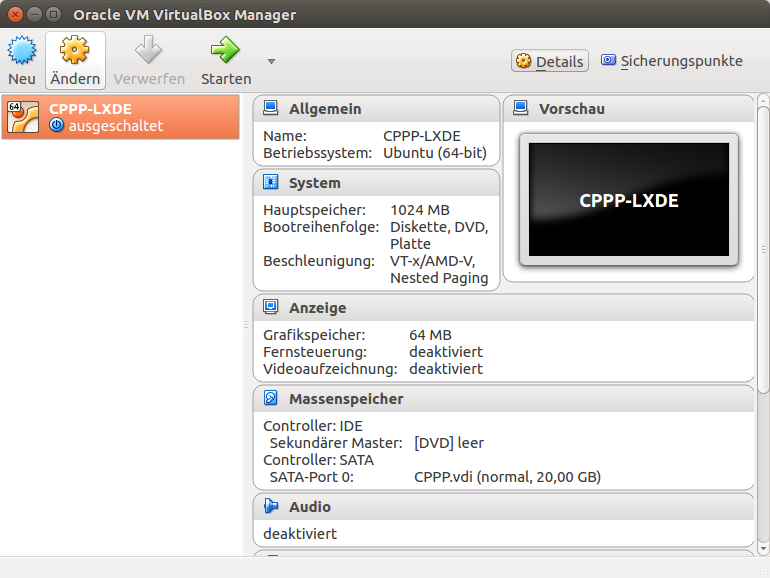
\includegraphics[width=0.6\textwidth]{figures/sf1.png}
\end{center}
\item Wähle links im Menü \textbf{Gemeinsame Ordner} aus. Klicke dann auf das Ordnersymbol mit dem grünen Plus, um einen neuen Shared Folder anzulegen.
\begin{center}
	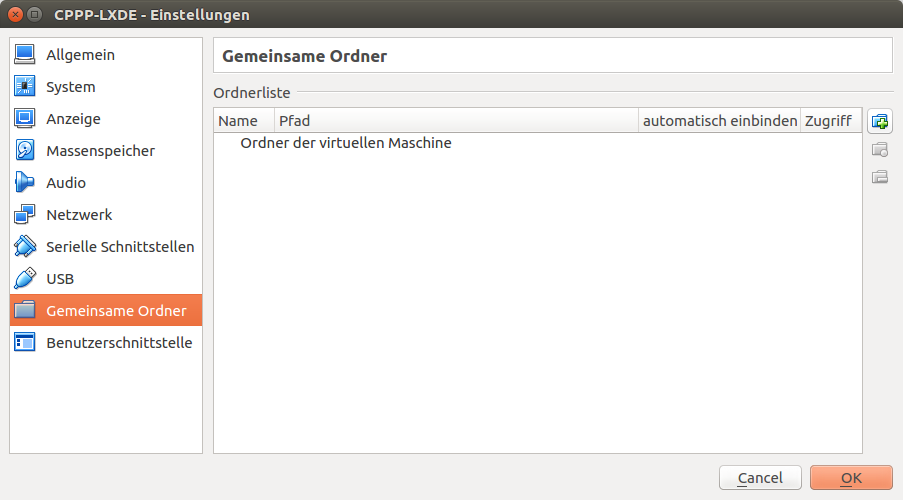
\includegraphics[width=0.6\textwidth]{figures/sf2.png}
\end{center}
\item Wähle den Ordner auf dem Host-PC aus und gib einen Namen ein.
Setzt ein Häkchen bei \textbf{Automatisch einbinden}.
\begin{center}
	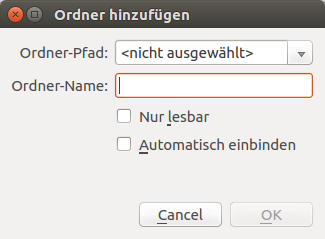
\includegraphics[width=0.3\textwidth]{figures/sf3.png}
\end{center}
\item Starte jetzt die VM neu. Im Dateimanager ist der Shared Folder in der linken Leiste zu sehen.
\end{itemize}

\section{Mikrocontroller}

\begin{center}
	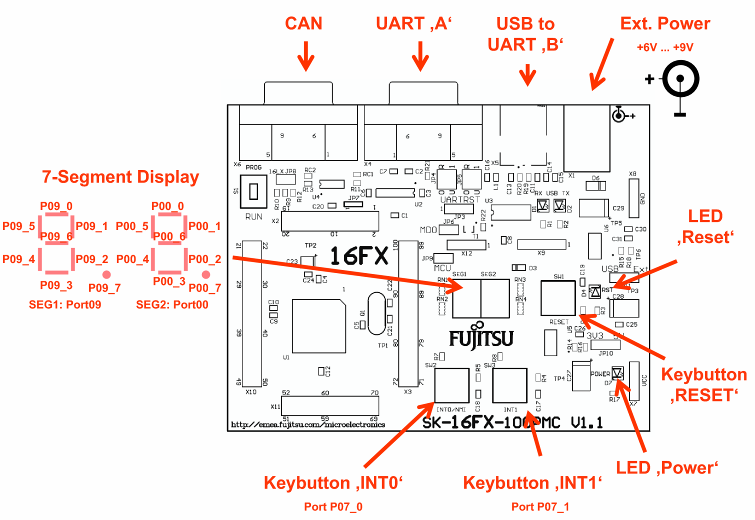
\includegraphics[width=0.6\textwidth]{figures/starterkit.png}
\end{center}


\subsection{Minimalprogramm}
Folgendes Programm bleibt unendlich lange in der \lstinline|for|-Schleife und führt bei jedem Durchgang eine Warteoperation durch.
Die \lstinline|#include|-Anweisung ist notwendig, um das Programm auf dem Mikrocontroller zu verwenden.
Es bietet Zugang zur Hardware, als auch Systemfunktionen wie zum Beispiel die Warteoperation.
% TODO wozu NOP?
\begin{lstlisting}
#include "mb96348hs.h"
void main(void) {
	for (;;) {
		__wait_nop();
	}
}
\end{lstlisting}
% - generisches Programm: main loop, Variablen müssen am Anfang des Scopes deklariert werden
% - Ansteuerung 7-Segment-Anzeige
% - Auslesen Taster
% - Auslesen Poti
% - Ansteuerung LCD

\end{document}
